\subsection{Progettazione database}
\label{subsec:database}
Il diagramma E-R (entità-relazione) mostrato in \hyperref[fig:db_only_dataset]{Figura \ref{fig:db_only_dataset}} espone lo schema concettuale del database.
\begin{figure}[H]
    \centering
    \resizebox{0.3\textwidth}{!}{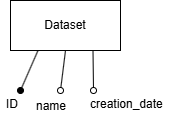
\includegraphics{Sezioni/ProgettazioneDettaglio/Immagini/db_only_dataset.png}}
    \caption{Schema concettuale database.}
    \label{fig:db_only_dataset}
\end{figure}

\subsubsection{Dataset}
\begin{itemize}
    \item \textit{ID}: valore numerico che identifica univocamente un dataset;
    \item \textit{Nome}: stringa che identifica univocamente il dataset;
    \item \textit{DataCreazione}: data di creazione del dataset;
\end{itemize}
